\usetikzlibrary{arrows.meta}
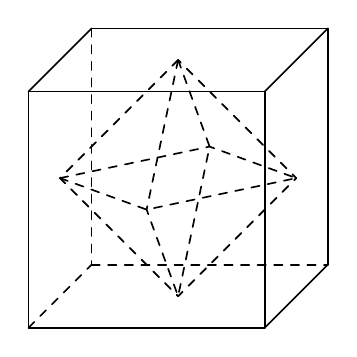
\begin{tikzpicture}[line width=0.6pt, line join=round, line cap=round]
\coordinate (F1) at (0,0);
\coordinate (F2) at (3,0);
\coordinate (F3) at (3,3);
\coordinate (F4) at (0,3);
\coordinate (B4) at (0.8,3.8);
\coordinate (B3) at (3.8,3.8);
\coordinate (B2) at (3.8,0.8);
\coordinate (B1) at (0.8,0.8);
\draw (F1) -- (F2) -- (F3) -- (F4) -- cycle;
\draw (F4) -- (B4);
\draw (F3) -- (B3);
\draw (F2) -- (B2);
\draw (B3) -- (B2);
\draw (B4) -- (B3);
\draw[dashed] (B4) -- (B1);
\draw[dashed] (B1) -- (B2);
\draw[dashed] (F1) -- (B1);
\coordinate (T) at (1.9,3.4);
\coordinate (Bo) at (1.9,0.4);
\coordinate (L) at (0.4,1.9);
\coordinate (R) at (3.4,1.9);
\coordinate (Fb) at (1.5,1.5);
\coordinate (Bk) at (2.3,2.3);
\draw[dashed] (T) -- (L) -- (Bo) -- (R) -- (T);
\draw[dashed] (T) -- (Fb) -- (Bo);
\draw[dashed] (T) -- (Bk) -- (Bo);
\draw[dashed] (L) -- (Fb) -- (R);
\draw[dashed] (L) -- (Bk) -- (R);


\end{tikzpicture}
